\chapter{Dodging Anvils: Exceptions \& Debugging}

\begin{figure}[h!]
    \centering
    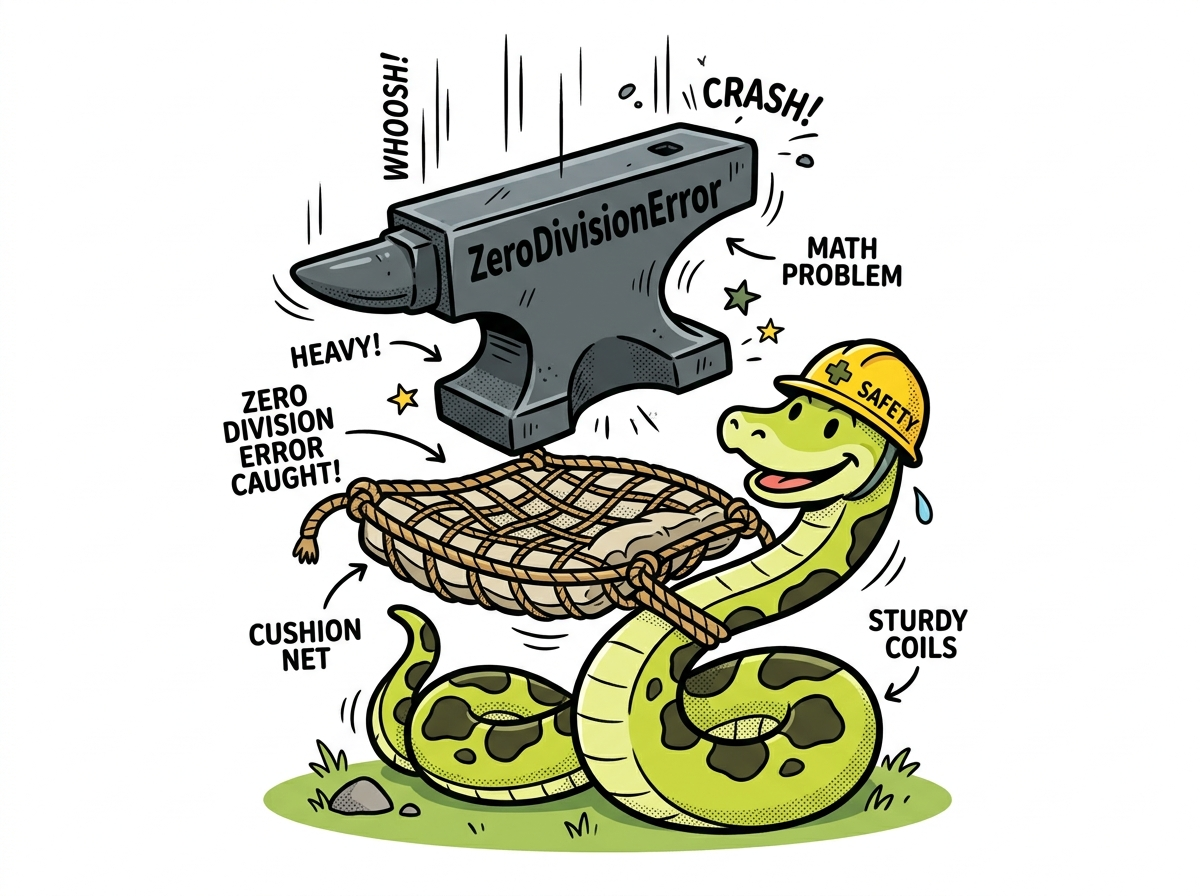
\includegraphics[width=0.75\textwidth]{images/ch6_falling_anvil.jpg}
    \caption{Exception handling is like wearing a hardhat and setting up safety nets to catch falling anvils gracefully.}
\end{figure}

\section{Bugs are Not Monstrous Errors --- They are Clues!}

Every programmer's code breaks. The difference between an amateur and a pro is that an amateur panics when seeing red error text, while a pro puts on detective glasses and reads the traceback!

Python exceptions occur when your code is syntactically valid, but an unexpected event happens at runtime (like dividing by zero or opening a file that doesn't exist).

\section{The Safety Net: \texttt{try} / \texttt{except} Blocks}

Instead of letting your program crash dramatically and scare the user, you can wrap risky code in a \texttt{try} block and catch errors gracefully in an \texttt{except} block.

\begin{pycode}{Catching Division by Zero}
def divide_cookies(total_cookies, people):
    try:
        per_person = total_cookies / people
        print(f"Everyone gets {per_person:.1f} cookies!")
    except ZeroDivisionError:
        print("WHOOPS! You cannot divide cookies among 0 people!")

divide_cookies(10, 2)
divide_cookies(10, 0)
\end{pycode}

\section{Catching Specific Exceptions}

Always catch specific exceptions rather than using a bare \texttt{except:}. Catching specific exceptions prevents you from accidentally swallowing critical system interrupts!

\begin{pycode}{Multiple Exception Handlers}
try:
    user_input = input("Enter a number: ")
    number = int(user_input)
    result = 100 / number
    print("Result:", result)
except ValueError:
    print("Error: That wasn't a valid integer!")
except ZeroDivisionError:
    print("Error: Cannot divide 100 by zero!")
except Exception as e:
    print(f"Unexpected Error: {e}")
\end{pycode}

\section{The Complete Rescue Team: \texttt{else} and \texttt{finally}}

- \textbf{\texttt{else}:} Runs ONLY if NO exceptions occurred in the \texttt{try} block.
- \textbf{\texttt{finally}:} Runs ALWAYS, no matter what happened (great for closing files or cleanup)!

\begin{pycode}{Full Try-Except-Else-Finally Structure}
try:
    print("Opening secret spellbook...")
    file_status = "OPEN"
    # Risky operation
    spell_level = 5
except NameError:
    print("Spell unknown!")
else:
    print("Spell level validated successfully!")
finally:
    file_status = "CLOSED"
    print(f"Cleanup complete. File status: {file_status}")
\end{pycode}

\section{Code Example: Bulletproof User Input Getter}

Here is a practical function pattern used in professional applications to repeatedly prompt users until they provide valid numerical input.

\begin{pycode}{Bulletproof Input Prompt}
def get_positive_integer(prompt_message):
    while True:
        try:
            val = int(input(prompt_message))
            if val <= 0:
                print("Error: Must be greater than 0!")
                continue
            return val
        except ValueError:
            print("Invalid input! Please type a whole number.")

# Simulated usage demo
# age = get_positive_integer("Enter your age: ")
print("Function pattern defined successfully!")
\end{pycode}

\begin{snakesnack}{Reading Stack Traces}
When Python prints a traceback:
1. Look at the **very last line** first! It tells you the exception name (\texttt{KeyError}, \texttt{TypeError}, \texttt{IndexError}).
2. Look at the line number mentioned right above it to pinpoint the exact line of code that triggered the anvil!
\end{snakesnack}

\section{Practice Problems \& Exercises}

Catch falling anvils in these 3 exception exercises!

\begin{snakelab}{Problem 6.1: Safe List Index Access (Easy)}
Write a function \texttt{safe\_get\_item(lst, index)} that returns the item at position \texttt{index}.
If the index is out of bounds, catch the \texttt{IndexError} and return \texttt{"Item Not Found"}.
Test with \texttt{colors = ["Red", "Green", "Blue"]} at index $1$ and index $99$!
\end{snakelab}

\begin{pycode}{Solution 6.1: Safe List Index Access}
def safe_get_item(lst, index):
    try:
        return lst[index]
    except IndexError:
        return "Item Not Found"

colors = ["Red", "Green", "Blue"]
print("Index 1:", safe_get_item(colors, 1))   # Green
print("Index 99:", safe_get_item(colors, 99)) # Item Not Found
\end{pycode}

\begin{snakelab}{Problem 6.2: Safe Dictionary Key Extractor (Medium)}
Write a function \texttt{safe\_dict\_lookup(dictionary, key, default\_value)}:
\begin{itemize}
    \item Try returning \texttt{dictionary[key]}.
    \item If a \texttt{KeyError} occurs, return \texttt{default\_value}.
\end{itemize}
Test looking up \texttt{"mana"} in \texttt{\{"hp": 100, "level": 5\}}.
\end{snakelab}

\begin{pycode}{Solution 6.2: Safe Dictionary Lookup}
def safe_dict_lookup(dictionary, key, default_value):
    try:
        return dictionary[key]
    except KeyError:
        return default_value

player = {"hp": 100, "level": 5}
mana = safe_dict_lookup(player, "mana", 50)
print(f"Player Mana: {mana}") # Returns default 50
\end{pycode}

\begin{snakelab}{Problem 6.3: Custom Range Validation Exception (Spicy)}
Write a function \texttt{set\_volume(level)}:
\begin{itemize}
    \item If \texttt{level} is not an integer, raise a \texttt{TypeError("Volume must be an integer!")}.
    \item If \texttt{level} is outside $0$ to $100$, raise a \texttt{ValueError("Volume must be between 0 and 100!")}.
\end{itemize}
Test calling \texttt{set\_volume(150)} inside a \texttt{try-except} block to catch and print the error message!
\end{snakelab}

\begin{pycode}{Solution 6.3: Custom Range Validation}
def set_volume(level):
    if not isinstance(level, int):
        raise TypeError("Volume must be an integer!")
    if level < 0 or level > 100:
        raise ValueError("Volume must be between 0 and 100!")
    print(f"Volume set to {level}%")

try:
    set_volume(150)
except (TypeError, ValueError) as err:
    print(f"Caught Expected Error: {err}")
\end{pycode}
